
\documentclass[utf8]{XDBAthesis}
% 图形文件的搜索路径
\def\allfiles{}
\def\pictures{}
\graphicspath{{../figures/}{../omnigraffle/}}
\numberwithin{algorithm}{chapter}
\floatname{algorithm}{算法}
\renewcommand{\algorithmicrequire}{\textbf{输入:}}
\renewcommand{\algorithmicensure}{\textbf{输出:}}
%\usepackage[nomarkers]{endfloat}

\begin{document}
%%----------------- 封面部分 ----------------- %%
      \class{031111}
    \schoolnumber{03111002}
    \title{大规模图数据库的相似性搜索}{}   %%题目超过14个字把剩下的放到第二个空
    \college{计算机学院}
    \major{计算机科学与技术}
    \author{贾新禹}
    \advisor{霍红卫}
    \maketitle
%%----------------- 前言部分 ----------------- %%
    
    \frontmatter
    \ifx\allfiles\undefined
\documentclass{XDBAthesis}
\def\pictures{}
\begin{document}
\else
\fi
\begin{abstract}
    随着科学技术的进一步发展,各种数据正以前所未有的速度增长着。如何有效存储,索引,搜索图数据成为一个日益显著的问题,因此图搜索已成为一个热门话题,并在大量领域都有应用,如分子化学,药物学,传感器网络,关系网络,XML文档等等。
    
    本文首先介绍了图搜索的基本概念,并探究了目前几个经典的图搜索算法,分析总结了这些算法优缺点。
    
    然后,针对精确搜索,本文以GraphGrep为基础提出了一种基于二次哈希开链法的新算法,解决了GraphGrep在索引定位中哈希容易产生冲突的问题,加快了搜索效率,并通过实验比较了两算法性能。
    
    其次,针对相似性搜索,本文结合G-Hash中小波匹配核函数和简化包表示提出了一种基于节点相似度的新算法,在效率不逊于G-Hash的基础上提高了匹配精度,降低了编码难度,并通过实验证明了此算法的正确性与可行性。
    
\keywords{图搜索\ \ \ 图精确搜索\ \ \ 图相似性搜索\ \ \ 二次哈希开链\ \ \ 节点相似度}
    
\end{abstract}
\begin{englishabstract}
With the further development of the science and technology, all kinds of data is growing at an unprecedented speed. How to effectively store, index and search figure data become an increasingly important problem, so the graph search has become a hot topic, and are used in many areas, such as molecular chemistry, pharmacology, sensor networks,human network, XML documents, and so on.

This paper first introduces the basic concept of graph search, and explore the current several classic graph search algorithm, these algorithms were analyzed advantages and disadvantages.

Then, in view of the accurate search, this paper put forward a new algorithm based on the secondary hash chain method,on the basis of the GraphGrep, to solve the GraphGrep hash prone to conflicts when index positioning, speed up the search efficiency, and compared the two algorithms performance through experiments.

Secondly, in view of the similarity search, this paper combine G-Hash wavelet matching kernel function and Reduced Bag to node similarity,then puts forward a new algorithm based on node similarity, the efficiency is not inferior to the G-Hash,But improved the precision of matching, reduces the coding difficulty, and through the experiment proves the correctness and feasibility of this algorithm.

\englishkeywords{Graph search \ \ \  Graph accurate Search \ \ \  Graph Similarity Search \ \ \ twice-hash chain\ \ \ node similarity}    
\end{englishabstract}



\ifx\allfiles\undefined
%\bibliographystyle{unsrt}
%\bibliography{main}
\end{document}
\fi
    \tableofcontents
%%----------------- 正文部分 ----------------- %%
    \mainmatter
    \pagestyle{content}
    \ifx\allfiles\undefined
\documentclass{XDBAthesis}
\begin{document}
\else
\fi
\chapter{引言}
\label{chap:introduction}
\section{研究背景与意义}
随着科学技术的进一步发展,我们正逐步从\emph{信息时代}走入\emph{数据时代}\cite{BigData},全球的数据量正在以一种前所未有的方式增长着。数据的迅速增长,在给人们带来便捷信息的同时,也带来了一个巨大的挑战——面对日益复杂的数据,传统的查询方法不再有效,无法快速检索出相关联数据。面对大量有意义的数据,无奈于查询手段的限制,只能将其简化再进行处理。现在的大数据现状就好似守着一座金山,却不知如何开采。为了进一步挖掘有效信息,加速查询速度,提高信息价值,各种数据查询技术便应运而生。

其中最为热门的就是图数据库的查询。图作为计算机科学中的一个数据结构,其数据表达能力较强,可以很好得表示

\ifx\allfiles\undefined
\renewcommand\refname{参考文献}
\bibliographystyle{unsrt}
\bibliography{main}
\end{document}
\fi
    \ifx\allfiles\undefined
\def\pictures{}
\documentclass{XDBAthesis}
\usepackage{todonotes}
\graphicspath{{../figures/}{../omnigraffle/}}
\begin{document}
\else
\fi
\chapter{背景知识}
\label{chap:background}
\section{图基本定义}
\begin{defn}[标号图]\cite{ghash}
    一个可以被四元组$G=(V,E,\Sigma,\lambda)$表示的图称为\emph{标号图(labeled graph)},其中$V$为有限的节点集合,$E$为有限的边集合$E\in V\times V$,$\Sigma$是标号集合,$\lambda$是一个标号函数用于给各个节点与边分配标号$\lambda :V\cup E\rightarrow\Sigma$。
\end{defn}
如图\ref{fg:label}就是一个包含六个节点的标号图。需要注意的是标号与标识的区别,标号是图的固有属性,标识只是为了方便使用人为添加的记号。在图\ref{fg:label}中,$v_i $就是标识,而$A,B,C,D$则是标号。

\begin{figure}[htp]
    \begin{minipage}{0.5\textwidth}
        \centering
        \ifx\pictures\undefined
\documentclass{article}
\usepackage{ctex}
\usepackage{tikz}

\begin{document}
\else
\fi
\ifx\hasdraw\undefined
\tikzstyle{vertex}=[circle,draw=black!25,minimum size=20pt,inner sep=0pt]
\tikzstyle{edge} = [draw,thick,-]
\def\hasdraw{}
\fi
    \begin{tikzpicture}[scale=2, auto,swap]
        \foreach \pos/\labels/\name/\lp in {{(0.5,1.5)/1/A/above}, {(1,1)/2/A/above}, {(0,1)/3/B/above},{(0,0)/4/C/left}, {(1,0)/5/C/right},{(2,1)/6/D/above}}
            \node[vertex] (\labels) at \pos [label=\lp:$v_{\labels}$]{$\name$};
        \foreach \source/ \dest  in {1/2,1/3,2/3,2/5,2/4,3/4,3/5,4/5,2/6}
                \path[edge] (\source) --  (\dest);
    \end{tikzpicture}
\ifx\pictures\undefined
\end{document}
\fi
        \figcaption{标号图}
        \label{fg:label}
    \end{minipage}%
    \begin{minipage}{0.5\textwidth}
        \centering
        \ifx\pictures\undefined
\documentclass{article}
\usepackage{ctex}
\usepackage{tikz}
\begin{document}
\else
\fi
\ifx\hasdraw\undefined
\tikzstyle{vertex}=[circle,draw=black!25,minimum size=20pt,inner sep=0pt]
\tikzstyle{edge} = [draw,thick,-]
\def\hasdraw{}
\fi
    \begin{tikzpicture}[scale=2, auto,swap]
        \foreach \pos/\labels/\name/\lp in {{(0.5,1.5)/1/A/above}, {(1,1)/2/A/above}, {(0,1)/3/B/above},{(0,0)/4/C/left}, {(2,1)/5/D/above}}
            \node[vertex] (\labels) at \pos [label=\lp:$v_{\labels}$]{$\name$};
        \foreach \source/ \dest  in {1/2,1/3,2/3,2/4,3/4,2/5}
                \path[edge] (\source) --  (\dest);
    \end{tikzpicture}
\ifx\pictures\undefined
\end{document}
\fi
        \figcaption{图\ref{fg:label}的子图}
        \label{fg:sub}
    \end{minipage}\hfill
\end{figure}
\begin{defn}[子图]
    如果一幅图$G=(V,E,\Sigma,\lambda)$和另一幅图$G'=(V',E',\Sigma',\lambda')$有1-1映射的关系$f:V\rightarrow V'$,那么图$G$就是$G'$的\emph{子图(subgraph)},用$G\in G' $表示。$f$需要满足以下几个条件:
\begin{itemize}
    \item 对于所有$v\in V,\lambda(v)=\lambda '(f(v))$
    \item 对于所有$(u,v)\in E,(f(u),f(v))\in E$
    \item 对于所有$(u,v)\in E,\lambda(u,v)=\lambda '(f(u),f(v)) $
\end{itemize}
\end{defn}
换言之,如果一幅图和另一幅图的节点标签,边关系,边标签能一一对应上,那么这副图就是另一幅图的子图。如图\ref{fg:sub}就是图一个\ref{fg:label}的子图,节点标签,边关系及边标签均可一一对应,只有标识可以不同。
\begin{defn}[超图]
    如果图$G$是图$G'$的子图,则$G'$是$G$的\emph{超图}。如对于图\ref{fg:label}和图\ref{fg:sub}而言,图\ref{fg:sub}是图\ref{fg:label}的子图,所以图\ref{fg:label}是图\ref{fg:sub}的超图。
\end{defn}

\begin{defn}[顶点的度]\cite{GraphAlgorithm}
    一个顶点$u$的\emph{度}数是与它相关联的边的数目,记做$degree(u)$。$degree(v_i )=|E(v_i )|,v_i \in V(i=1,2,...,n)$,图\ref{fg:label}中$v_2 $的度$degree(v_2 )=5$,图\ref{fg:sub}中$v_2 $的度为$degree(v_2)=4$。
\end{defn}
\begin{defn}[图的尺寸]\cite{g13}
    一般由图中节点数$|V(G)|$定义。因此图\ref{fg:label}的\emph{尺寸(size)}为6,图\ref{fg:sub}为5。
\end{defn}
\begin{defn}[路径]\cite{GraphAlgorithm}
在图$G(V,E)$中,若从顶点$v_i$出发,沿着一些边经过一些顶点$v_{p1},v_{p2},...,v_{pm}$,到达顶点$v_j $,则称顶点序列$(v_{i},v_{p1},v_{p2},...,v_{pm},v_{j})$为从顶点$v_i $到$v_j $的一条\emph{路径(path)}。如在图\ref{fg:label}中,$(v_{1},v_{2},v_{5})$就是一条$v_1 $到$v_5 $的路径。  
\end{defn}
\begin{defn}[图的同构]\cite{g13}
给定图$G$和图$G'$,若$G'$满足$G'\equiv_{iso}G$,则称$G$与$G'$是\emph{同构图}。$G'\equiv_{iso}G$同构,当且仅当存在一个双射函数$f:V(G)\leftrightarrow V(G')$,其满足下列条件:
\begin{itemize}
    \item 对于所有$v\in V,\lambda(v)=\lambda '(f(v))$
    \item 对于所有$u,v\in V,(u,v)\in E\Leftrightarrow (f(u),f(v))\in E$
    \item 对于所有$(u,v)\in E,\lambda(u,v)=\lambda '(f(u),f(v)) $
\end{itemize}  
\end{defn}
如图\ref{fg:iso},图$G_1$和图$G_2$就是一组同构图,顶点标号$A\leftrightarrow X,B\leftrightarrow Y,C\leftrightarrow Z$,$G_1$中的边与$G_2$的边也形成双射关系。
\begin{figure}[htb]
    \centering
    \subfigure[$G_1$]{
        \ifx\pictures\undefined
\documentclass{article}
\usepackage{ctex}
\usepackage{tikz}
\begin{document}
\else
\fi
\ifx\hasdraw\undefined
\tikzstyle{vertex}=[circle,draw=black!25,minimum size=20pt,inner sep=0pt]
\tikzstyle{edge} = [draw,thick,-]
\def\hasdraw{}
\fi
\begin{tikzpicture}[scale=0.5, auto,swap]
    \foreach \pos/\labels/\name/\where in {{(3,6)/1/A/right}, {(0,3.5)/2/B/above}, {(1,0)/3/C/left},{(5,0)/4/A/right}, {(6,3.5)/5/B/above}}
        \node[vertex] (\labels) at \pos [label=\where:$v_{\labels}$]{$\name$};
    \foreach \source/ \dest  in {1/2,2/3,3/4,4/5,5/1}
            \path[edge] (\source) --  (\dest);
\end{tikzpicture}
\ifx\pictures\undefined
\end{document}
\fi
    }
    \subfigure[$G_2$]{
        \ifx\pictures\undefined
\documentclass{article}
\usepackage{ctex}
\usepackage{tikz}
\begin{document}
\else
\fi
\ifx\hasdraw\undefined
\tikzstyle{vertex}=[circle,draw=black!25,minimum size=20pt,inner sep=0pt]
\tikzstyle{edge} = [draw,thick,-]
\def\hasdraw{}
\fi
\begin{tikzpicture}[scale=0.5, auto,swap]
    \foreach \pos/\labels/\name/\where in {{(3,6)/1/X/right}, {(0,3.5)/2/X/above}, {(1,0)/3/Y/left},{(5,0)/4/Y/right}, {(6,3.5)/5/Z/above}}
        \node[vertex] (\labels) at \pos [label=\where:$v_{\labels}$]{$\name$};
    \foreach \source/ \dest  in {1/3,2/4,3/5,4/1,5/2}
            \path[edge] (\source) --  (\dest);
\end{tikzpicture}
\ifx\pictures\undefined
\end{document}
\fi
    }
    \caption{图的同构}
    \label{fg:iso}
\end{figure}

\section{图存储表示方式}
图存储表示方法有很多种,常用的有2种:\emph{邻接矩阵(Adjacency Matrix)}和\emph{邻接表(Adjacency List)}。本节还将介绍一种新颖的图表示方法\emph{简化包表示(Reduced Bag Representation)}\cite{ghash}。
\subsection{邻接矩阵}
 在邻接矩阵存储方法中,除了一个记录各个顶点信息的顶点数组外,还有一个表示各个顶点之间关系的矩阵,称为\emph{邻接矩阵}\cite{GraphAlgorithm},设$G(V,E)$是一个具有$n$个顶点的图,则图的邻接矩阵是一个$n\times n$的二维数组,用$Edge[n][n]$表示,定义为:
\begin{equation}
    Edge[i][j]=\left\{
    \begin{aligned}
        1 & , if (i,j)\in E \\
        0 & , else    
    \end{aligned}\right. 
\end{equation}

%\todo{增加邻接矩阵图} 

\subsection{邻接表}
    \emph{邻接表}\cite{GraphAlgorithm}就是将同一个顶点发出的边连接在同一个称为边链表的单链表中。边链表的每个节点代表一条边,称为边节点。每个边节点有两个域:该边终点的序号以及下一个边节点的指针。
    
%\todo{增加邻接表图}   
%    \begin{figure}[htb]
%        \centering
%        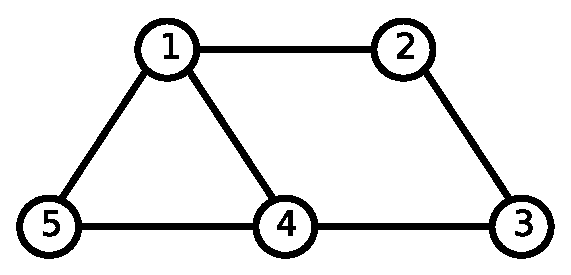
\includegraphics[width=0.4\textwidth]{../figures/BasicGraph_GraphExample}
%        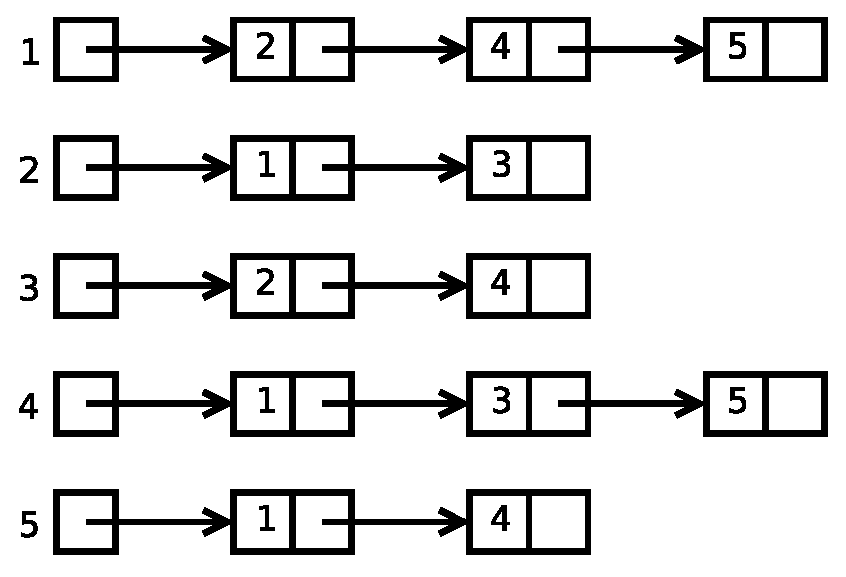
\includegraphics[width=0.4\textwidth]{../figures/BasicGraph_AdjacencyListRepresentation}
%        \caption{邻接表}
%        \label{fg:adjacencyList}
%    \end{figure}
\subsection{包表示法}
\emph{包表示法}是Wang教授等人在\emph{G-Hash}\cite{ghash}中提出的一种方法。这种方法的主要思想是将图中的各个节点特征提取出来形成一个列表,然后将这些特征就作为每个节点的标识。这样整幅图就变成了一个字符串的包,也就是一组字符串。通常,我们用这个节点的标号和其邻接节点的不同标号数目为特征。例\ref{exmp:bag1}所示就是一个常用的包表示方法
\begin{exmp}
    表\ref{tb:bagr1}是图\ref{fg:label}的包表示。我们以节点标号和其邻接节点各个标号的个数作为特征,因此有五个特征:本身标号,A,B,C,D分别的个数。所以加上第一列的标识,表一共有六列。而一共有六个不同节点,所以有六行。我们以$v_3 $为例,详细说明下抽取特征的步骤。首先$v_3 $的标号是B,所以Label为B,然后和$v_3$邻接的共有四个节点,分别是$v_1 ,v_2 ,v_4 ,v_5 $,其标号分别为$A,A,C,C$所以$\#A=2,\#C=2$,其余为0。节点$v_3 $的包表示就是“B,2,0,2,0”,如表\ref{tb:bagr1}所示。需要注意一点的是,包表示不仅仅这一种表示方法,对于选取什么样的特征并没有限制。不过特征必须是离散的,这样才可以用字符串表示。
    \label{exmp:bag1}
\end{exmp}


\begin{table}[htb]
    \centering
    \begin{tabular}{c|c|c|c|c|c}
        Nodes & Label & \#A & \#B & \#C & \#D \\ \hline
        $v_1$ & A & 1 & 1 & 0 & 0 \\ \hline
        $v_2$ & A & 1 & 1 & 2 & 1 \\ \hline
        $v_3$ & B & 2 & 0 & 2 & 0 \\ \hline
        $v_4$ & C & 1 & 1 & 1 & 0 \\ \hline
        $v_5$ & C & 1 & 1 & 1 & 0 \\ \hline
        $v_6$ & D & 1 & 0 & 0 & 0 \\ \hline
    \end{tabular}
    \tabcaption{图\ref{fg:label}的包表示}
    \label{tb:bagr1}
\end{table}
    
\section{图搜索类型}
根据图之间的包含关系,可将图查询搜索技术分为子图查询和超图查询;根据图搜索的精确程度,可以将其分为精确搜索和相似性搜索\cite{g13}。
\begin{defn}[子图查询]\cite{FSD}
子图查询的问题为:对于给定的一个查询图,返回图数据库中所有查询图的超图。给定一个图数据库$GD$和一个查询图$q$,子图查询的目的是找出在$GD$中所有包含$q$或者$q$的同构的图的集合,最后返回该超图集合$Q$。$Q=\{G|G\in GD\wedge q\subseteq G\}$。
\end{defn}
\begin{defn}[超图查询]\cite{ssosc}
超图查询的问题为:对于给定的一个查询图,返回图数据库中所有查询图的子图。给定一个图数据库$GD$和一个查询图$q$,超图查询的目的是找出在$GD$中所有以$q$为超图的图的集合,最后返回该子图集合$Q$。$Q=\{G|G\in GD\wedge q\supseteq G\}$。    
\end{defn}

\begin{figure}[htb]
    \centering
    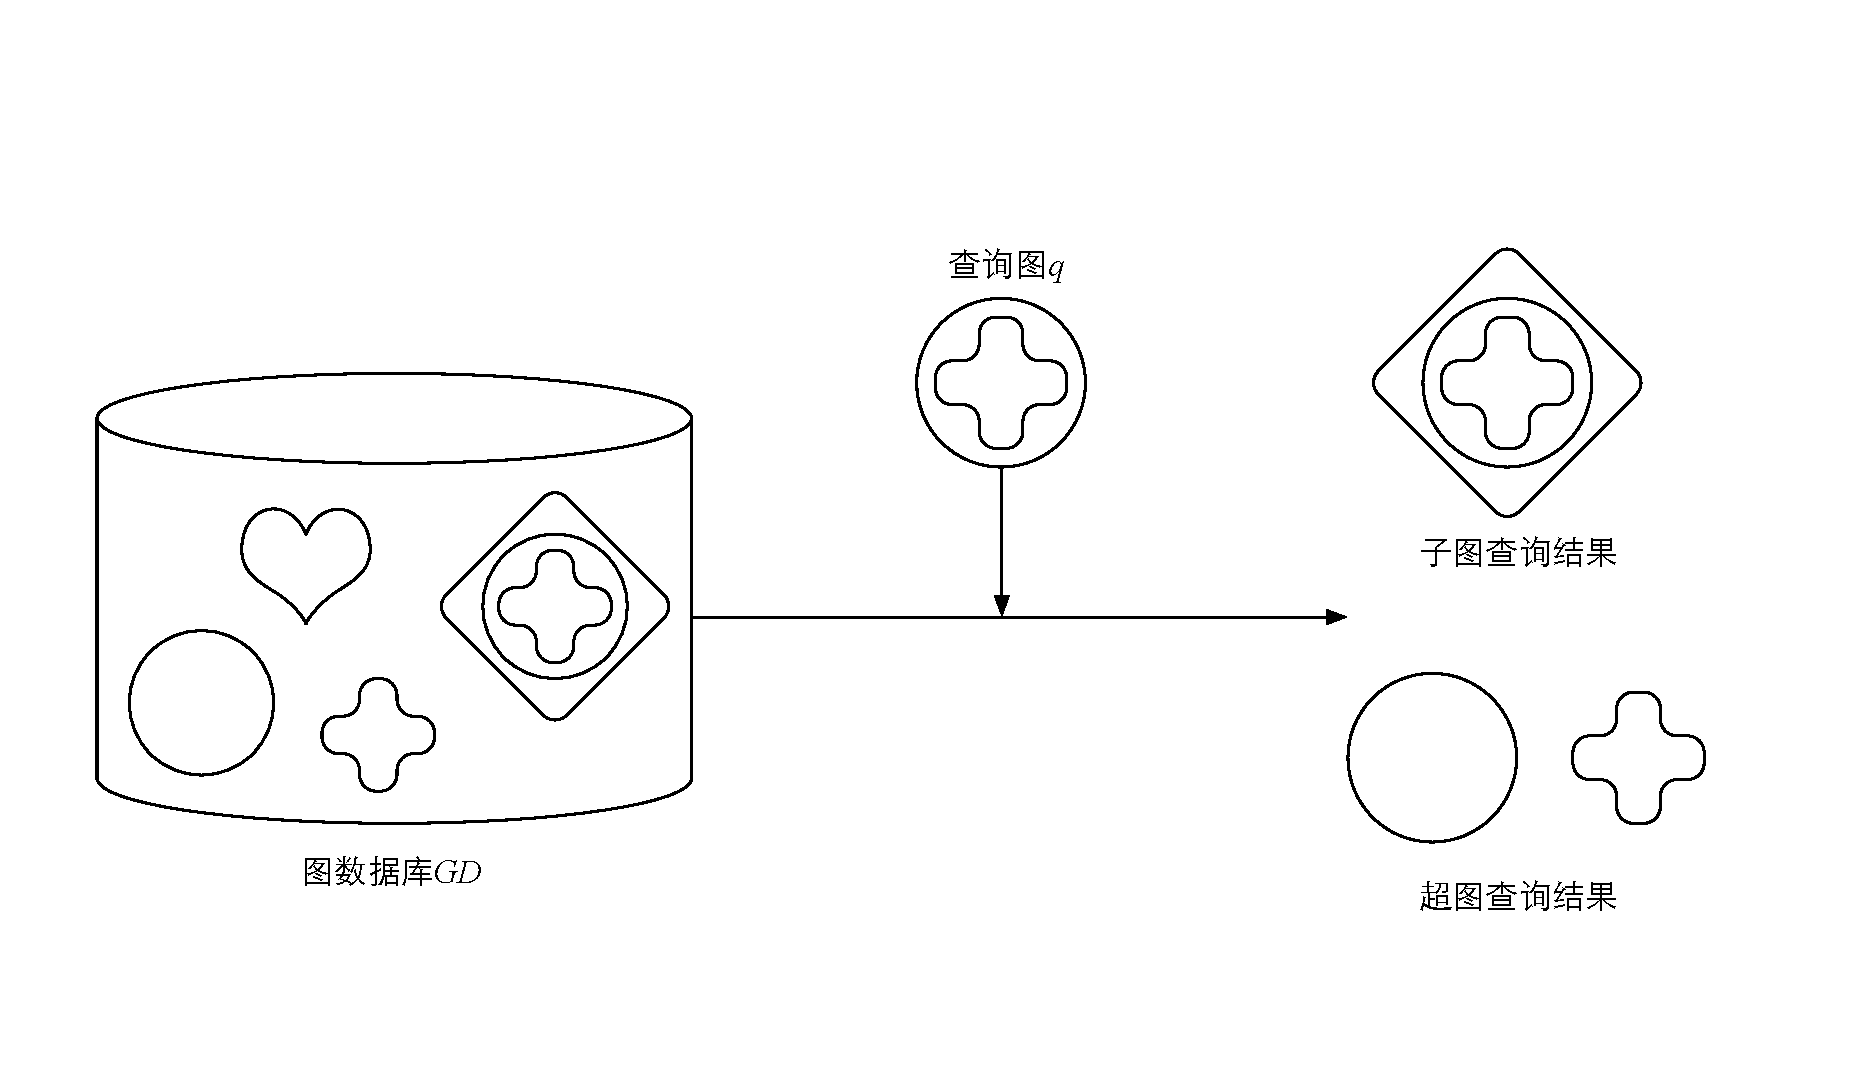
\includegraphics[width=0.75\textwidth]{Database.eps}
    \caption{子图查询与超图查询}
    \label{fg:subsup}
\end{figure}

如图\ref{fg:subsup}就是同一个查询$q$在同一数据库中子图查询和超图查询的不同结果。



\begin{defn}[精确搜索]\cite{gIndex}
图精确搜索,又称精确查询,是这样定义的:对于给定数据库$G_D =\{G_1 ,G_2 ,...,G_n \}$,查询图$q$,返回$G_D $中与$q$具有子图同构的图集合。具体可以分为子图查询和超图查询。如图\ref{fg:simacu}所示,对于精确查询查询图$q$的结果就是$\{G_1 ,G_2  \}$
\end{defn}


\begin{defn}[相似性搜索]\cite{gghash}
图相似性搜索,又称近似查询,是这样定义的:对于给定数据库$G_D =\{G_1 ,G_2 ,...,G_n \}$,查询图$q$,返回$G_D $中与$q$距离小于预设阀值的图集合。如图\ref{fg:simacu}所示,对于近似查询查询图$q$的结果就是$\{G_1 ,G_2 ,G_3 ,G_4 \} $
\end{defn}

显然,近似查询中相似性度量方法和预设的阀值决定了结果集的大小。阀值越大,结果集越大;阀值越小,结果集越少。当阀值为零是,其结果应该与精确查询一致。

\begin{figure}[htb]
    \centering
    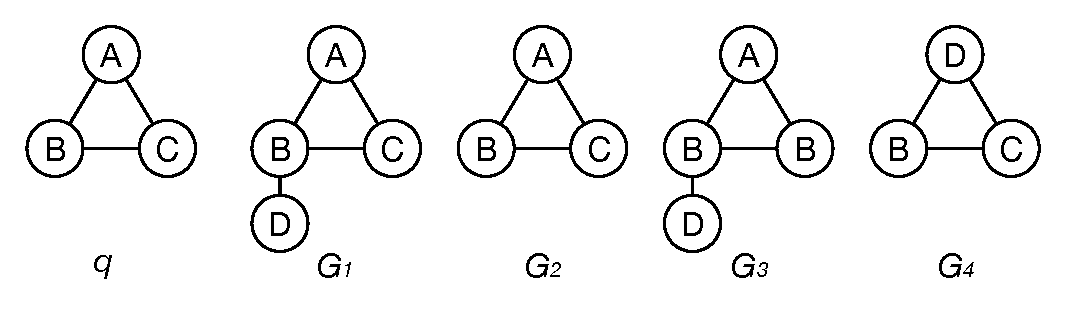
\includegraphics[width=0.8\textwidth]{2last}
    \caption{精确查询与相似查询}
    \label{fg:simacu}
\end{figure}

常见的相似性度量方法有两种,一种方法是\emph{编辑距离(edit distance)}.\emph{编辑距离}就是我们将图$G$通过一系列操作(如增删点边,重新标号等)变换为另一个图$G^{'}$所需的操作数。面对不同的需求,我们可以通过给不同操作分配不同的权值,然后计算权值和作为距离,来使度量更精确。编辑距离是一种非常直观的图相似性测度方法,但是我们很难计算(实际上,这是个NP-hard问题)。还有一种常用方法是\emph{最大公共子图(maximal common subgraph)}\cite{mcs},顾名思义,这里就不详细说明了。

\ifx\allfiles\undefined
%\renewcommand\refname{参考文献}
\bibliographystyle{unsrt}
\bibliography{main}
\end{document}
\fi
    \ifx\allfiles\undefined
\documentclass{XDBAthesis}
\begin{document}
\else
\fi
\chapter{经典图查询算法}
\label{chap:classic}
本章将详细介绍几种经典的图查询算法。由于基本的图查询模式均为“过滤-验证”,所以要提高查询效率,只能从两方面优化。一是过滤阶段优化,二是验证阶段优化。众所周知,图是结构画的数据,目前并没有一个统一高效的索引机制可以实现较好的查询结果。因此大多数学者都会在过滤阶段选用不同的索引方式来得到更好的查询结果。而在验证阶段,由于图同构是个NP-hard问题,所以验证会消耗大量时间。如何快速检测同构,或将同构转为其他非复杂多项式的一半问题也是学者们关心的一个热点课题。本章介绍的几种查询方法均为过滤阶段的优化。
\section{图精确查询算法}
本节将详细介绍子图查询中的\emph{GraphGrep}算法\cite{graphgrep}和\emph{gIndex}算法\cite{gIndex}。
\subsection{GraphGrep算法}
2002年ShaSha教授等人提出了\emph{GraphGrep}算法。GraphGrep算法是基于特征索引方法中的第一个经典算法,它采取典型的“过滤-验证”框架,GraphGrep算法中只讨论过滤阶段。由于基于结构的算法中对图的顺序扫描代价太高,GraphGrep提出基于路径的过滤方法,来减少候选集大小。

其算法的主要流程是这样的:
\begin{enumerate}
    \item 构造索引:首先将节点和边利用哈希存成两个二维表作为未来筛选用特征之一,然后枚举图数据库中所有长度不大于$l_p $的路径$v_0 ,v_1 ,v_2 ,...,v_k ,( k\leq l_p ,\forall i\in [1,k-1],(v_i ,v_i+1)\in E) $,然后将这些路径与图的关系存为一个二维表作为索引。表的每一行代表每一个图,每一列为一个路径,利用简单哈希确定路径对于行号,每一个单元格代表在该图包含该路径几条,如表\ref{tb:grepIndex}所示。

\begin{table}[htb]
    \centering
    \begin{tabular}{|c|c|c|c|}
        \hline
        Key&$g_1 $&$g_2 $&$g_3 $ \\ \hline
        h(CA)&1&0&1 \\ \hline
        ...&&&\\ \hline
        h(ABAB)&2&2&0 \\
        \hline
    \end{tabular}
    \caption{GraphGrep索引}
    \label{tb:grepIndex}
\end{table}

    \item 解析查询: 如同图数据库,首先将节点和边利用哈希存成两个二维表,然后枚举查询中的所有长度不大于$l_p $的路径,哈希存在一个列表中。
    \item 数据库过滤: 
        \begin{enumerate}
            \item 利用节点信息过滤:如果查询图中的某一节点在数据库中一图里未出现,则此图一定不会包含查询图,因此可以删去。
            \item 利用边信息过滤:同节点过滤,如果某条边未出现,则一定不会包含查询图,可删去。
            \item 利用路径个数进行过滤:如果查询图中某一路径个数大于数据库中一图的此路径个数,则此图一定不会包含查询图,可以从候选集中删去。
        \end{enumerate}
    \item 子图查询: 利用标号进行路径合成,从候选集中删去所有未能成功合成的候选图。剩下的就是GraphGrep算法返回的候选集。后续再加以图同构验证即可得到最终子图查询结果。
    
    \todo{详细合成过程}
\end{enumerate}






\ifx\allfiles\undefined
\bibliographystyle{unsrt}
\bibliography{main}
\end{document}
\fi
    \ifx\allfiles\undefined
\documentclass{XDBAthesis}
\def\pictures{}
\numberwithin{algorithm}{chapter}
\floatname{algorithm}{算法}
\renewcommand{\algorithmicrequire}{\textbf{输入:}}
\renewcommand{\algorithmicensure}{\textbf{输出:}}
\begin{document}
\else
\fi
\chapter{基于二次哈希开链法的图精确搜索}
\label{chap:graphgrep}
由于传统算法在利用哈希表存储索引中多采用简单哈希,容易产生冲突问题,导致构建索引效率较低。本章在路径索引的基础上,探究了不同哈希方法对算法速度的影响,并提出一种基于二次哈希开链法的精确搜索算法,来减少图搜索中的过滤阶段的耗时,以提高搜索速度。本章将先介绍下现有的哈希算法,然后详细介绍基于二次哈希开链法搜索的搜索方法包括作为此算法验证方法用的子图同构算法\emph{ULLMANN}\cite{ullmann}。最后是实验结果与分析。

\section{常用哈希方法}
本节将介绍三种常用的解决哈希冲突的方法,开放定址法,开链法,再哈希法。

\subsection{开放定址法}
开放定址法\cite{datastruct}是一种常用的处理冲突方法,公式如\eqref{eq:open}所示
\begin{equation}
    H_i =(H(key)+d_i )MOD\ m\ \  \ i=1,2,...,k(k\leq m-1)
    \label{eq:open}
\end{equation}

其中,$H(key)$为哈希函数;$m$为哈希表表长,$d_i $为增量序列,可有以下三种取法:
\begin{enumerate}
    \item $d_i =1,2,3,...,m-1$,称线性探测再散列;
    \item $d_i =1^2 ,-1^2 ,2^2 ,-2^2 ,3^2 ,...,\pm k^2 ,(k\leq m/2 ) $,称为二次探测再散列;
    \item $d_i =$伪随机数序列,称为伪随机探测再散列。
\end{enumerate}
\subsection{开链法}
开链法又称链地址法\cite{datastruct},是将所有关键字为同义词的记录存储在同一线性链表中。
\subsection{再哈希法}
\begin{equation}
    H_i =RH_i (key)\ i=1,2,...,k
    \label{eq:twice}
\end{equation}
再哈希法\cite{datastruct}如公式\eqref{eq:twice}所示,$RH_i $均是不同的哈希函数,即在同义词产生地址冲突时计算另一个哈希函数地址,直到冲突不再发生。
\section{基于二次哈希开链法的搜索算法}
本方法同\emph{GraphGrep}算法\cite{graphgrep},都是基于路径的精确子图搜索算法。算法基本流程如下:(1)遍历图数据库中图的路径,(2)利用双哈希构建索引,(3)遍历查询图路径,(4)利用基本索引特征先验剪枝,(5)路径合成进一步筛选候选集,(6)子图同构确定最终结果。下面我们将分小节详细说明这些步骤。
\subsection{数据库路径遍历}
首先,对于每个数据库我们设定一个路径长度的上限$l_p $,$l_p $越大意味着可记录的路径越长,索引集合也会相应增加。随后对于数据库中的每幅图,我们用深度优先搜索遍历每个节点,遍历最大深度为$l_p $,并记录遍历过程中经过的每一条路径,存成一个列表,用于下一步构建索引。
\subsection{二次哈希开链法索引构建}
双哈希是再哈希的一种,其利用两个哈希函数来构造哈希探测序列,大大降低了地址冲突概率。但是传统上,双哈希方法实质上也是开放定址法的一种,也就是如果所需节点数目大于$Mod$时,将完全无法表示。这完全不符合图数据库实际情况,因为作为一个通用算法,我们无法预先确定数据库中最大图的节点数。因此,本文将双哈希和开链法相结合提出了一个变形的双哈希算法,即\emph{二次哈希开链法}来进行哈希定址。

二次哈希开链法就是只进行一次双哈希,然后再有冲突就利用开链法解决。双哈希函数公式如\eqref{eq:hash_e}。
\begin{equation}
    h(key)=(h_1 (key)+ h_2 (key))\%Mod
    \label{eq:hash_e}
\end{equation}

其中$h_1 ,h_2 $为两个不同的哈希函数,$Mod$为哈希函数取模值,一般为一个小于但最接近存储空间大小的素数。当$h_1 (key)$发生冲突时,再用$h_2 (key)$的值作为偏移量来进行探测。如果再有冲突则进行开链法,存成链表。

根据二次哈希开链法的特点,本文设计了一种将路径字符串映射到哈希表的算法,如算法\ref{algo:hashcode}所示。而访问时函数则不需重新设计,直接用开链法原有函数即可。

\begin{algorithm}
\caption{二次哈希编码}
\label{algo:hashcode}
\begin{algorithmic}[1]
    \Require 路径字符串 $path\_string$
    \Ensure 哈希编码 $code$
    \Function {hash}{$path\_string$}
        \State $code \gets h_1 (key)\%Mod$
        \If {$code$有冲突}
            \State $code \gets (code+h_2 (key))\%Mod$
        \EndIf
        \State \Return{$code$}
    \EndFunction     
\end{algorithmic}
\end{algorithm}

在二次哈希开链法中哈希函数可以自选,不过我们推荐选取算法\ref{algo:hashfunction}中的两个函数作为$h_1 ,h_2 $,经过实验这两个函数对于字符串哈希这两个效果最好。

\begin{algorithm}
\caption{哈希函数}
\label{algo:hashfunction}
\begin{algorithmic}[1]
    \Require 字符串 $String$
    \Ensure 哈希编码 $code$
    \Function {$h_1 $}{$String$}\Comment{BKDRHash}
        \State $char \gets (string.first)$
        \State $code \gets 0$
        \While {$char \neq 0 $}
            \State $code \gets code<<6+char$
            \State $char \gets (char.next)$
        \EndWhile
        \State \Return{$(code\&0\times 7FFFFFFF)\%Mod$}
    \EndFunction
    \Function {$h_2 $}{$String$}\Comment{APHash}
        \State $char \gets (string.first)$
        \State $code \gets 0$
        \State $i \gets 0 $
        \While {$char \neq 0 $}
            \If{$i$为偶数}
                \State $code \gets (code\oplus ((code<<7)\oplus char\oplus (code>>3))$
            \Else
                \State $code \gets (code\oplus (\sim ((code<<11)\oplus char\oplus (code>>5)))  $
            \EndIf
            \State $char \gets (char.next)$
        \EndWhile
        \State \Return{$(code\&0\times 7FFFFFFF)\%Mod$}
    \EndFunction          
\end{algorithmic}
\end{algorithm}

\emph{BKDRHash}运算简单,速度快,所以作为第一次哈希函数。\emph{APHash}不易冲突,所以作为第二次。

通过哈希存储,我们可以很便捷得获得各图包含的路径关系表,我们将其存到文件中作为索引,分离查询与建库,进行离线查询加速查询速度。

\subsection{查询图路径遍历}
我们对查询图也像数据库中的图一样进行拆分,以$l_p $为路径最大长度遍历出所有路径。然后同样存成一个哈希表,记录着每一条路径出现了几次。为进一步搜索做准备。不过和数据库路径遍历有所不同的是,查询图的遍历过程中需要记录不同路径中相同的节点,这个可以通过在路径中添加特定标签实现。
\subsection{先验剪枝}
    在介绍本算法的先验剪枝步骤之前,我们先介绍一下\emph{包含逻辑规则(inclusion logic)}。
    \begin{defn}[包含逻辑]\cite{inclusionlogic}
        对于给定的标号图$g_1 ,g_2 $,和$g_1 $的一个子图$g'$,若$g_1 $是$g_2 $的子图,则$g'$必定是$g_2 $的子图$(g_1 \subseteq g_2 ) \Rightarrow (g' \subseteq g_2  )$。反之,若$g'$不是$g_2 $的子图,则$g_1 $也不可能是$g_2 $的子图$(g' \not\subset g_2  )\Rightarrow (g_1 \not\subset g_2 )$    
    \end{defn}
    从包含逻辑规则中,我们可以得知如果查询图$g_1 $中的子图$g'$不是数据图$g_2 $的子图,那么$g_2 $就不可能是$g_1 $的超图,因此可以放心得把$g_2 $从候选集中删去。这就大大加速了“过滤-验证”框架中过滤阶段的过滤速度。
    
    在本算法中,我们从三个方面进行了先验剪枝来缩小索引集个数。三个方面分别是(i)节点,(ii)边,(iii)路径。如果查询图中的某个节点个数大于数据图中的,那么数据图自然不会包含查询图。如果查询图中有数据图中没有的边,那么自然这幅数据图也不合要求。如果查询图中某条路径的个数大于数据图,那么因为包含逻辑规则,这幅数据图也当从候选集中删去。
    
    经过这三步筛选过程,候选集将会大大减少,降低了后文所述路径合成和子图同构所需时间。
\subsection{路径合成}
当完成先验剪枝后,候选集已经相对较小,但是并没有达到最好的情况。我们可以通过路径合成确定其中很多的合理性。路径合成的复杂度远远小于子图同构,因此最后对候选集做一次路径合成可以大大降低最终复杂度。
路径合成,顾名思义就是将多条路径进行合成,具体而言就是将多个有着公共节点的路径合成到一起,通过判定其是不是相同节点来筛选候选集。我们采用的是遍历的方法,只进行两两合成,然后逐一比对。如例\ref{exmp:pathcombine}所示。
\begin{exmp}
    假设有路径$\bar{A}B\underbar{C}\bar{A} $和$\underbar{C}B$,其中有相同标记的节点均为同一节点,即在本例中两个$A$是同一节点和两个$C$也是同一节点。
    \label{exmp:pathcombine}
    \begin{enumerate}
        \item 现在假设数据库中有四幅图,其路径信息如下所示,数字代表节点标识:
        $$
        \begin{aligned}
            g_1 &:ABCA={(1,0,3,1)}\ CB={(3,2)}\\
            g_2 &:ABCA={(1,2,3,1)}\ CB={(3,2)}\\
            g_3 &:ABCA={(1,0,3,4)}\ CB={(3,2)}\\
            g_4 &:ABCA={(1,0,4,1)}\ CB={(3,2)}\\
        \end{aligned}
        $$
        \item 在路径合成前,我们就可以利用节点信息删去$g_3$,因为$g_3$的$ABCA$中两个$A$一个是1,一个是4,并非同一节点。
        \item 我们将ABCA和CB合成,我们知道其中两个$A$是统一节点,两个$C$是同一节点,而两个$B$不是。我们得到合成结果:
        $$
        \begin{aligned}
            g_1 &:ABCACB={(1,0,3,1),(3,2)}\\
            g_2 &:ABCACB={(1,2,3,1),(3,2)}\\
            g_4 &:ABCACB={(1,0,4,1),(3,2)}\\
        \end{aligned}
        $$
        \item  显然,$g_2$不满足条件,因为它的两个$B$也是一个节点,$g_4$也不满足,因为其两个$C$不是同一节点。所以筛选集中只剩下$g_1$。
    \end{enumerate}    
\end{exmp}
可见,通过路径合成,我们大大缩小了候选集,降低了下一步子图同构所需的计算量,加速了整个算法。

\subsection{子图同构}
子图同构作为算法最后的验证部分,承担着对于整个算法正确性把关的责任,也同样是个需要消耗大量运算量的部分。由于子图同构是个$NP-hard$问题,所以目前仍没有一种快速的解法。我们选用经典算法\emph{ULLMANN}算法\cite{ullmann}来解决这个问题。下面我们将大致介绍下UllMANN算法。

ULLMANN算法是Ullmann教授1976年提出的一种经典图同构算法,其本质是基于一个深度优先搜索树。其算法流程如图\ref{fg:ullmanchart}所示。首先,根据查询图节点的出入度从数据图中找出候选集。随后,再根据每个节点的邻接节点对候选集进行筛选。最后,通过深度优先搜索,一一遍历配对,寻找匹配点。例\ref{exmp:ullmann}就是一个子图同构的完整过程。
\todo{补充Ullmann图和例子}
\begin{figure}
    \caption{Ullmann算法流程图}
    \label{fg:ullmanchart}
\end{figure}
\begin{exmp}
    \label{exmp:ullmann}    
\end{exmp}


\section{实验结果与分析}
\subsection{实验环境}
本文提出算法的实验环境为CPU Intel Core i7,主频为1.7 GHz,内存为8 GB 1600 MHz DDR3,硬盘为128GB SSD,操作系统为Mac OS X Yosemite 10.10.3;所有算法均用C语言在clang 600.0.56环境编译完成。
\subsection{实验数据分析}
实验数据全采用真实数据,为DTP提供的AIDS数据集。可从以下网址得到:\url{https://wiki.nci.nih.gov/display/NCIDTPdata/AIDS+Antiviral+Screen+Data}。我们从其数据库中随机抽取了1000,2000,4000,8000,16000个图作为我们的查询集合。所有实验运行10次取平均值。

实验结果如图\ref{fg:THCBuild},\ref{fg:THCRun}所示,THC为Twice Hash Chain(二次哈希开链法)的缩写。我们测试了不同最大长度$l_p $下两个算法的表现。
\begin{figure}[htb]
    \centering
    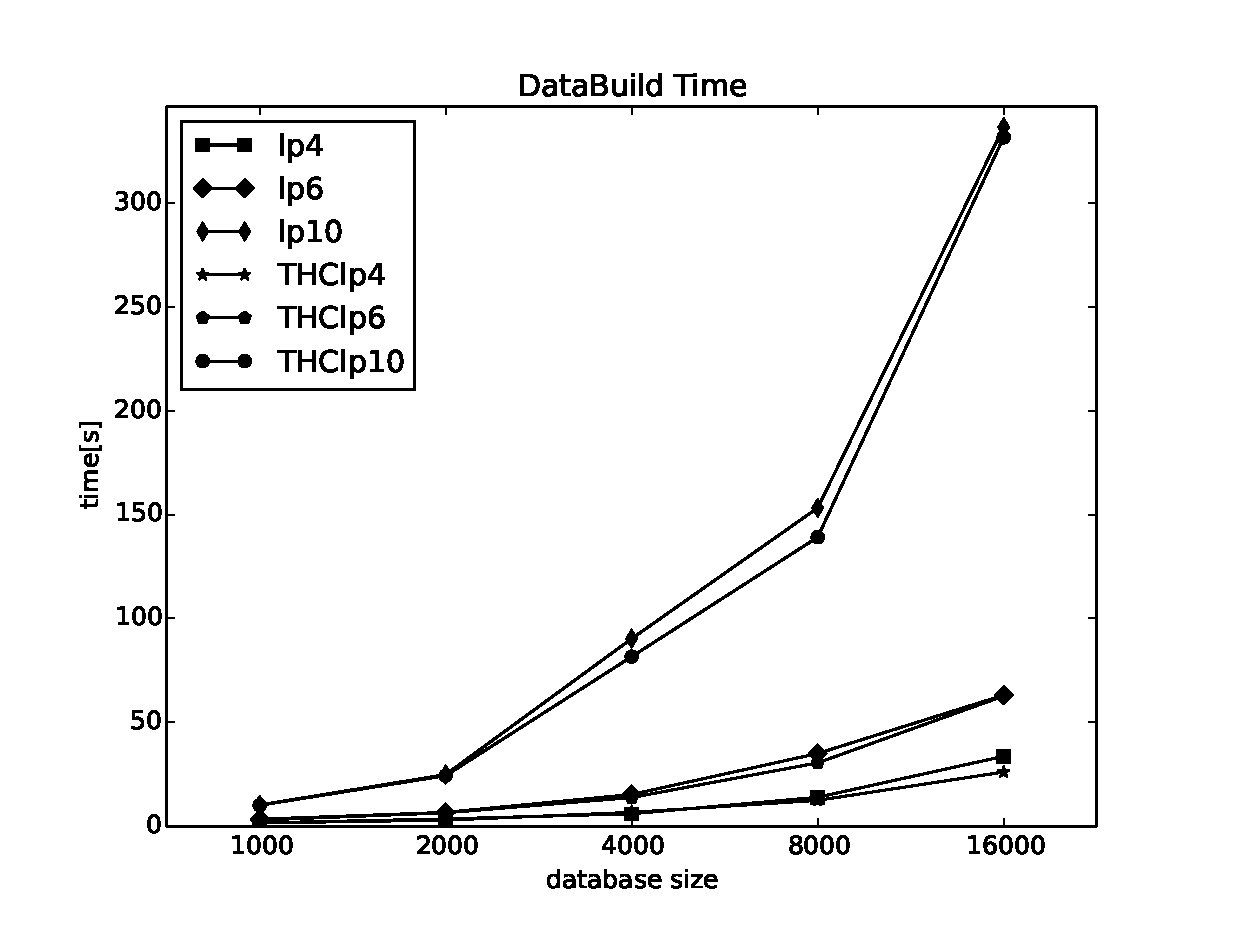
\includegraphics[width=0.5\textwidth]{../figures/THC/BuildCompare_4_6_10}%
    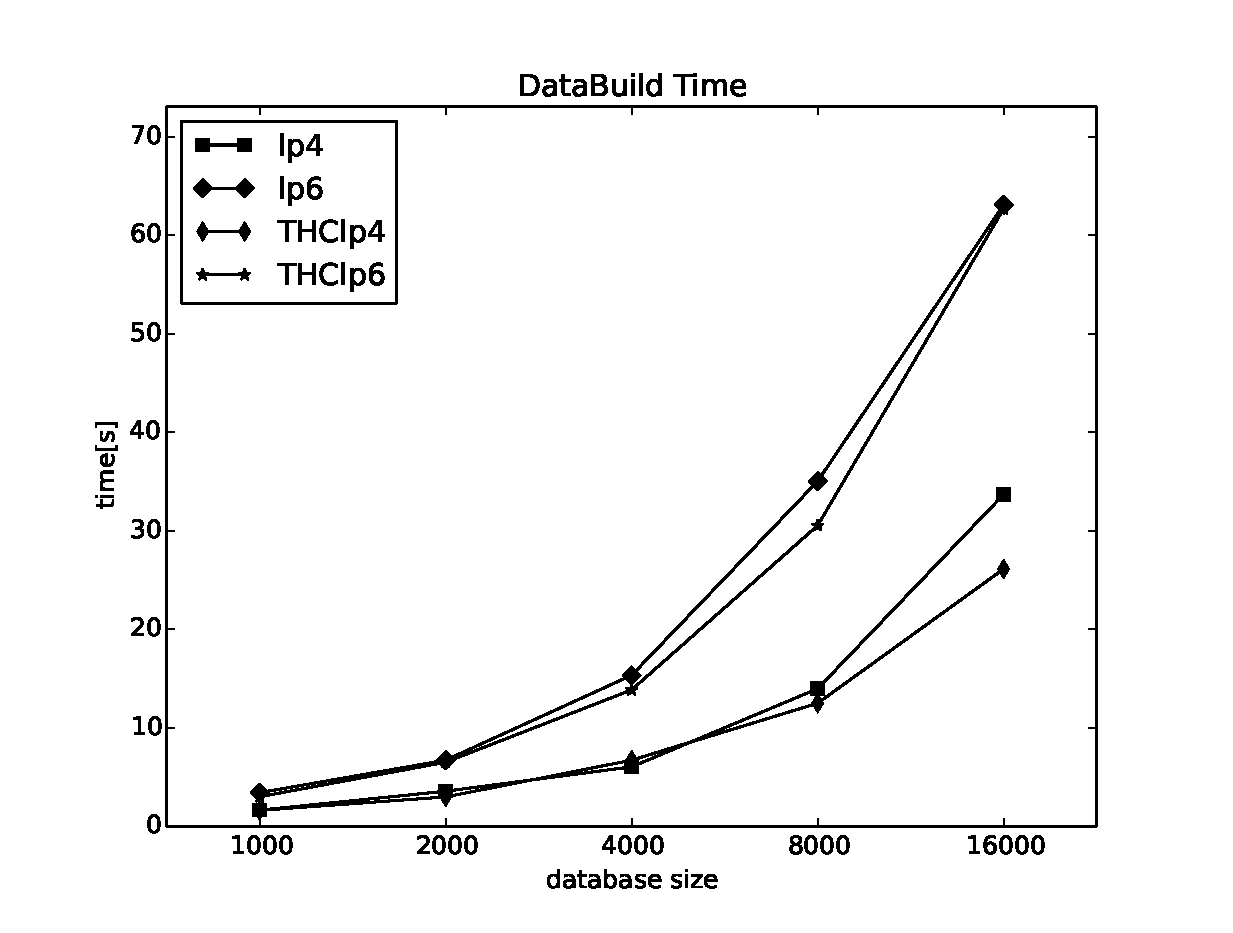
\includegraphics[width=0.5\textwidth]{../figures/THC/BuildCompare_4_6}
    \caption{建库时间比较}
    \label{fg:THCBuild}
\end{figure}
\begin{figure}[htb]
    \centering
    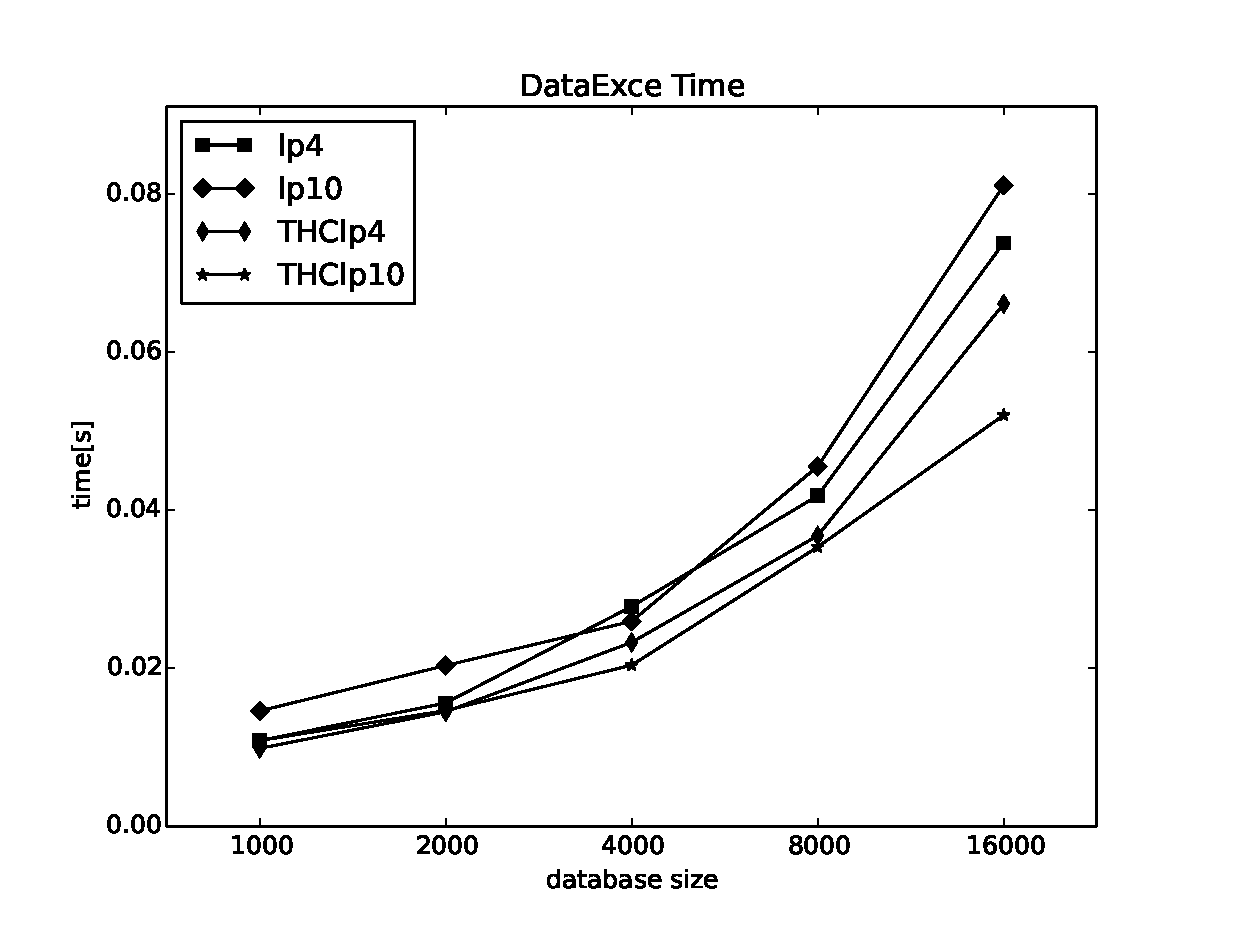
\includegraphics[width=\textwidth]{../figures/THC/ExceCompare_4_10}
    \caption{运行时间比较}
    \label{fg:THCRun}
\end{figure}

由图可知,二次哈希开链的确有效减少了冲突,提高了建库速度与查询速度。

\ifx\allfiles\undefined
\bibliographystyle{unsrt}
\bibliography{main}
\end{document}
\fi
    \ifx\allfiles\undefined
\documentclass{XDBAthesis}
\def\pictures{}
\begin{document}
\else
\fi
\chapter{基于节点相似度的图相似性搜索}
\label{chap:gHash}
由前文可知,图数据能表示复杂的数据结构,在诸多领域也得到了广泛应用。从基本的生物,化学的分子结构,到交通网络,人际关系网都可以用图来建模。而对于图数据库的索引也自然成为了热点问题。

上一章我们介绍了精确子图搜索方法,但是由于真实情况下图数据库具有信息不完整,含有杂质等情形,精确搜索容易出现各种不匹配问题,难以得到我们想要的结果。同时,对于查询图的完整信息有时查询者也并不了解。所以相似性搜索的实际应用领域更加广泛。对于实际应用,相似性搜索的研究意义远超过了精确搜索。

传统的图相似性算法虽然运行效率已较为理想,但是编码上过于复杂,也无法做到对所有图数据库良好适配。所以本章我们提出了一种性能上不输于传统算法,但是实现更为简单,并且无需复杂设计即可适用于大量图数据库的基于节点相似度的通用型算法。本章将首先详细介绍下一些相关概念,然后介绍下我们算法的具体思路并给出详细的代码设计方案,最后给出对于真实数据的实验结果与分析。
\section{相关概念}
本节主要介绍下下文介绍算法时会用到的一些概念,包括小波图匹配核函数,G-Hash中的图相似度定义,节点相似度定义三部分。
\subsection{小波图匹配核函数}
\emph{小波图匹配核函数(Wavelet Graph matching kernel)}\cite{ghash}是Wang等人在G-Hash算法中提出的,用于度量图相似度的一个核心函数。其思想是先通过压缩每个节点周围邻接节点的属性信息,然后应用非递归线性核去计算图之间的相似度。这个方法包含两个重要的概念:\emph{h-hop邻域}和\emph{离散小波变换}。用$N_h (v)$标记一个节点$v$的\emph{h跳邻域},代表一个距离节点$v$最短距离是$h$跳(跳过$h$个节点,也就是$h+1$的曼哈顿距离)的节点集合。\emph{离散小波变换}涉及到一个小波函数的定义,见下文公式\ref{eq:wavelet} ,也用到了$h$跳邻域。
\begin{equation}
    \psi_{j,k}=\frac{1}{h+1}\int_{j/(k+1)}^{(j+1)/(k+1)}\varphi(x)dx
    \label{eq:wavelet}
\end{equation}
$\varphi(x)$代表\emph{Haar}或者\emph{Mexican Hat}小波函数,$h$是在将$\varphi(x)$在$[0,1)$区间上分成$h+1$个间隔后的第$h$个间隔,$j\in[0,h]$。
基于以上两个定义,我们现在可以将小波分析用在图上了。我们用小波函数来计算每个节点的局部拓扑和。公式\eqref{eq:wm}展示了一个小波度量方法,记做$\Gamma_h (v)$,以图$G$中的一个节点$v$为例。
\begin{equation}
    \Gamma_h (v)=C_{h,v}\times\sum_{j=0}^k \psi_{j,k}\times\bar{f}_j (v)
    \label{eq:wm}
\end{equation}
其中,$C_{h,v}$是一个归一化因子
\begin{equation}
    C_{h,v}=(\sum_{j=0}^h \frac{\psi_{j,h}^2 }{|N_h (v)|})^{-1/2},
\end{equation}
$\bar{f}_{j}(v)$是离节点$v$最远距离为$j$的原子特征向量的平均值
\begin{equation}
    \bar{f}_{j}(v)=\frac{1}{|N_{j}(v)|}\sum_{u\in N_{j}(v)}f_u
\end{equation}
$f_u $表示节点$v$的特征向量值。这样的特征向量值只会是下面四种中的一种:定类,定序,定距,定比。对于定比和定距特征值,直接在上述的小波分析时代入其值即可得到局部特征值。对于定类和定序节点特征,我们首先建立一个直方图,然后用小波分析提取出特征值。在节点$v$分析完成后,我们可以得到一个节点列表$\Gamma^h (v)=\{\Gamma_{1}(v),\Gamma_{2}(v),...,\Gamma_{h}(v)\}$,我们称其为小波测度矩阵。用此方法我们可以将一个图转换为一个节点向量集合。因为小波变换有明确的正负区域,所以这些小波压缩特征可以表示出局部的邻接节点和距离较远的邻接节点的差异。因此,通过小波变换,一幅图的结构化信息可以压缩成节点特征。从而我们可以忽略拓扑结构来专心于节点匹配。核函数就是建立在这些集合上的,我们以图$G$和$G'$为例,图匹配核函数是这样的
\begin{gather}
    k_{m}(G,G')=\sum_{(u,v)\in V(G)\times V(G')}K(\Gamma^{h}(u),\Gamma^h (v) ), \\
    K(X,Y)=e^{\frac{-\|X-Y\|_{2}^{2}}{2}}.
\end{gather}
WA方法是一种很好的利用核函数进行图相似度定义的方法。但是这个方法有一个问题,就是小波匹配核的总时间复杂度是$O(m^2 )$,核矩阵的是$O(n^2 \times m^2 )$,$n$是数据库图个数,$m$是平均节点个数。这意味着,当数据库尺寸增加时,计算时间将大幅度增加。

\subsection{G-Hash中的图相似性定义}
图相似性有很多种定义方式有很多,第\ref{chap:background}章中介绍的\emph{图编辑距离}和\emph{最大公共子图}就是两种常用的图相似度度量方法。

G-Hash中是利用核函数计算两图相似性的。公式\ref{eq:ghashDistance}就是两图相似度距离的定义。
\begin{equation}
\begin{split}
    &d(G,G')=\sqrt{\|\phi(G)-\phi(G')\|_{2}^{2}}\\
              &=\sqrt{\langle\phi(G)-\phi(G'),\phi(G)-\phi(G')\rangle}\\
              &=\sqrt{\langle\phi(G),\phi(G)\rangle+\langle\phi(G'),\phi(G')\rangle-2\langle\phi(G),\phi(G')\rangle}\\
              &=\sqrt{k_{m}(G,G)+k_{m}(G',G')-2k_{m}(G,G')}
\end{split}
\label{eq:ghashDistance}
\end{equation}

公式中$k_{m}(G,G)$代表图$G$和其本身的核函数值,$k_{m}(G',G')$是图$G'$及其本身的值,$k_{m}(G,G')$就是图$G$和$G'$的。

\begin{equation}
k_{m}(G,G')=\sum_{v\in G',u\in simi(v)}K(\Gamma^{h}(u),\Gamma^{h}(v))
\end{equation}

$simi(v)$是一个包含着图$G$和节点$v$哈希到同一个位置的节点集合。我们用以下的解码方式来获取包含这些节点的图号和节点号。

显然,仅利用相似点对而非所有点对来计算两图相似度可以节约很多运算时间。因此为了增加准确度,相似的节点应该被哈希到相邻的位置。在图很大(如大于40)时,我们也要计算相邻位置的节点。

因此在核函数计算时我们只考虑相似点对,在使用RBF核的情况下,$K(\Gamma^{h}(u),\Gamma^{h}(v))\approx1$,所以公式(2)可以写成
\begin{equation}
    K(G,G')\approx\sum_{v\in G',u\in simi(v)}1=\sum_{v\in G'}|simi(v)| 
\end{equation}

$|simi(v)|$是在$simi(v)$中的节点数目。这意味着我们只需要数据图$G$中和查询$G'$相似的点个数,其和就是我们要求的核。同理,我们可以这样计算每个图与其自己的核。显然,每个图与自己的核就是节点数目。

所以公式\ref{eq:ghashDistance}最终变成公式\ref{eq:ghashfinal},其中$|V_{G}|$代表图$G$的节点数。
\begin{equation}
    d(G,G')=\sqrt{|V_{G}|+|V_{G'}| -2\sum_{v\in G'}|simi(v)| }
    \label{eq:ghashfinal}
\end{equation}

%在完成上述操作后,我们会得到一个相似度列表,其每一个值都对应这一个数据库中的图与查询图的相似度,通过对这个列表排序,我们就可以得到对于给定的查询的$K-NNs$。
\subsection{节点相似度}
在上一节我们介绍了G-Hash中的图相似性的定义。其中有参数$simi(v)$代表与节点$v$相似的节点,但是何为相似,这个很难定义。G-Hash算法在这边根据不同图数据库构建了不同类型的哈希,来保证相似的节点都在相邻位置。而这在实际应用中很是困难。因此我们提出了\emph{节点相似度}这一概念。我们用查询图每个节点和数据图中每个节点的节点相似度作为$simi(v)$的值。
\begin{defn}[节点相似度]
    用\emph{简化包(Reduced Bag)}表示的两个节点字符串之间的相似度节点相似度称为\emph{节点相似度}。
\end{defn}
因为简化包表示的字符串实质上是一个向量,如$'a,1,0,1'$就可以看做一个向量$\vec{A}=(a,1,0,1) $,所以对于字符串的距离,也就是节点相似度,可以用公式\eqref{eq:stringdis}计算。
\begin{equation}
    simi(A,B)=\frac{\vec{A}\times \vec{B}}{||\vec{A}|\times |\vec{B}||} \leq 1
    \label{eq:stringdis}
\end{equation}
其中,$|\vec{A}|$表示$\vec{A}$的模,$simi(A,B)$永远是小于等于1的,值越大代表越为相似,为1代表两个节点特征完全一样。
\section{基于节点相似度的图相似性搜索}
本算法和G-Hash\cite{ghash}基本类似,只是在查询过程计算相似度时没有利用哈希特征找到相似的节点,而是利用节点相似度来计算相似度。这样避免了由于哈希函数选取不当造成的相似节点不在靠近位置的问题。用普通的枚举虽然理论复杂度从$O(1)$变为了$O(n)$但是提高了查询准确度,并且由于哈希存在冲突,而实际图节点一般最多为千个等情况,我们算法的运行效率并不比G-Hash低,甚至在某些情况下会略好于G-Hash算法,而且编码难度也大大降低。本节将从数据库构建,查询过程,数据库维护,编码设计四个方面详细说明我们提出的基于节点相似度的图相似性搜索算法。
\subsection{数据库构建}
首先统计数据库中的不同标号数目,然后将数据库中的每幅图都用简化包表示,选取节点标号和与其直接连接的各标号个数作为特征值。归一化后变成字符串,利用红黑树建立Bag编号与字符串的对应关系。之所以选用红黑树而不是哈希表是因为对于纯字符串结构红黑树的表现要好于哈希表。然后再以Bag编号为图,图序号为列建立一个二维表,每个值代表在此图中此种节点有几个。最终数据库如图\ref{fg:ghashdatabase}所示。
\todo{补充一张红黑树的图,一张数据库table}
\begin{figure}
    \caption{数据库示例}
    \label{fg:ghashdatabase}
\end{figure}
\subsection{查询前K个相似图}
首先,我们参考G-Hash的图距离函数定义了我们的基于节点相似度的图距离函数,即公式\eqref{eq:ghashfinalreal}。\todo{修改公式引用改为eqref}
\begin{equation}
     d(G,G')=\sqrt{|V_{G}|+|V_{G'}| -2\sum_{v\in G',u\in G}simi(v,u)}
     \label{eq:ghashfinalreal}
\end{equation}
当我们得到一个查询图$G'$时,我们也用简化包将其表示,得到节点字符串集。然后利用公式\eqref{eq:ghashfinalreal}计算查询图和数据库中每副图的距离。随后将结果排序,取出最小的K个即为与查询图最相似的K个图。

\subsection{数据库维护}
当需要增删图的时候,会出现两种情况:(i)增删图对标号个数没有影响,即没有因为添加图而添加新的标号,也没有标号因为删除图而不被使用, (ii)增删图对标号个数有影响,即因为添加图而引入了新的标号,或者因为删除图而有的标号不再有图使用。当出现(i)情况时,只需要添加一列或者删除一列即可。当出现(ii)情况时,则需要重新建立数据库索引,不过无需每次出现都重新建立,每5-10次重建一次即可。
\subsection{代码设计}
本算法的实现非常简单,不需要任何复杂数据结构,只需要三个类即可实现。类图设计如图\ref{fg:ghashdesign}所示。
\begin{figure}
    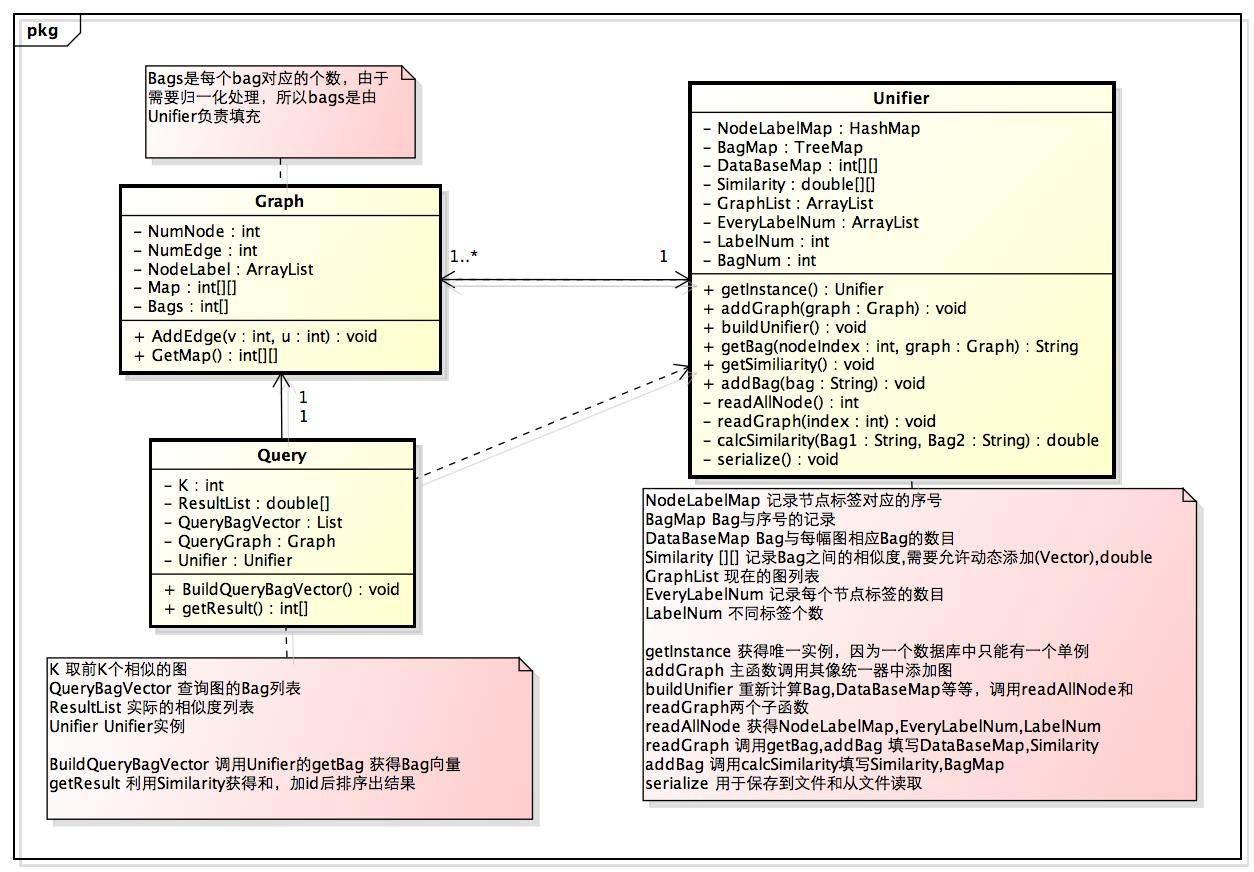
\includegraphics[width=\textwidth ]{../figures/G-Hash-pkg}
    \caption{基于节点相似度的图相似性搜索设计类图}
    \label{fg:ghashdesign}
\end{figure}

其中,$Graph$为一个最小单元即一个图,对外提供一些基本数据访问方法。$Unifier$顾名思义,是个用于归一化的类,也是数据库类,负责建库,增删图,和数据查询时一些算法定义,像获取简化包表示,图相似度计算就是靠这个类实现的。$Query$是一个查询,通过调用$Unifier$实现查询过程,最后输出查询结果。结果表现为图的id列表。我们还给$Unifier$添加了序列化接口,实现建库查询分离,加速查询过程。

由上可见,基于节点相似度的图相似算法实现非常方便,可运用在大量环境中。


\section{实验结果与分析}
\subsection{实验环境}
本文提出算法的实验环境为CPU Intel Core i7,主频为1.7 GHz,内存为8 GB 1600 MHz DDR3,硬盘为128GB SSD,操作系统为Mac OS X Yosemite 10.10.3;所有算法均用Java语言在JDK1.7u71环境编译完成。
\subsection{实验数据分析}
实验数据全采用真实数据,为DTP提供的AIDS数据集。可从以下网址得到:\url{https://wiki.nci.nih.gov/display/NCIDTPdata/AIDS+Antiviral+Screen+Data}。我们从其数据库中随机抽取了1000,2000,4000,8000,16000个图作为我们的查询集合。数据集平均每幅图有41条节点,48条边。由于未能联系到原作者,实验中用于对照的G-Hash算法也是我们根据G-Hash论文\cite{ghash}自行仿写的。
\begin{figure}[htb]
    \centering
    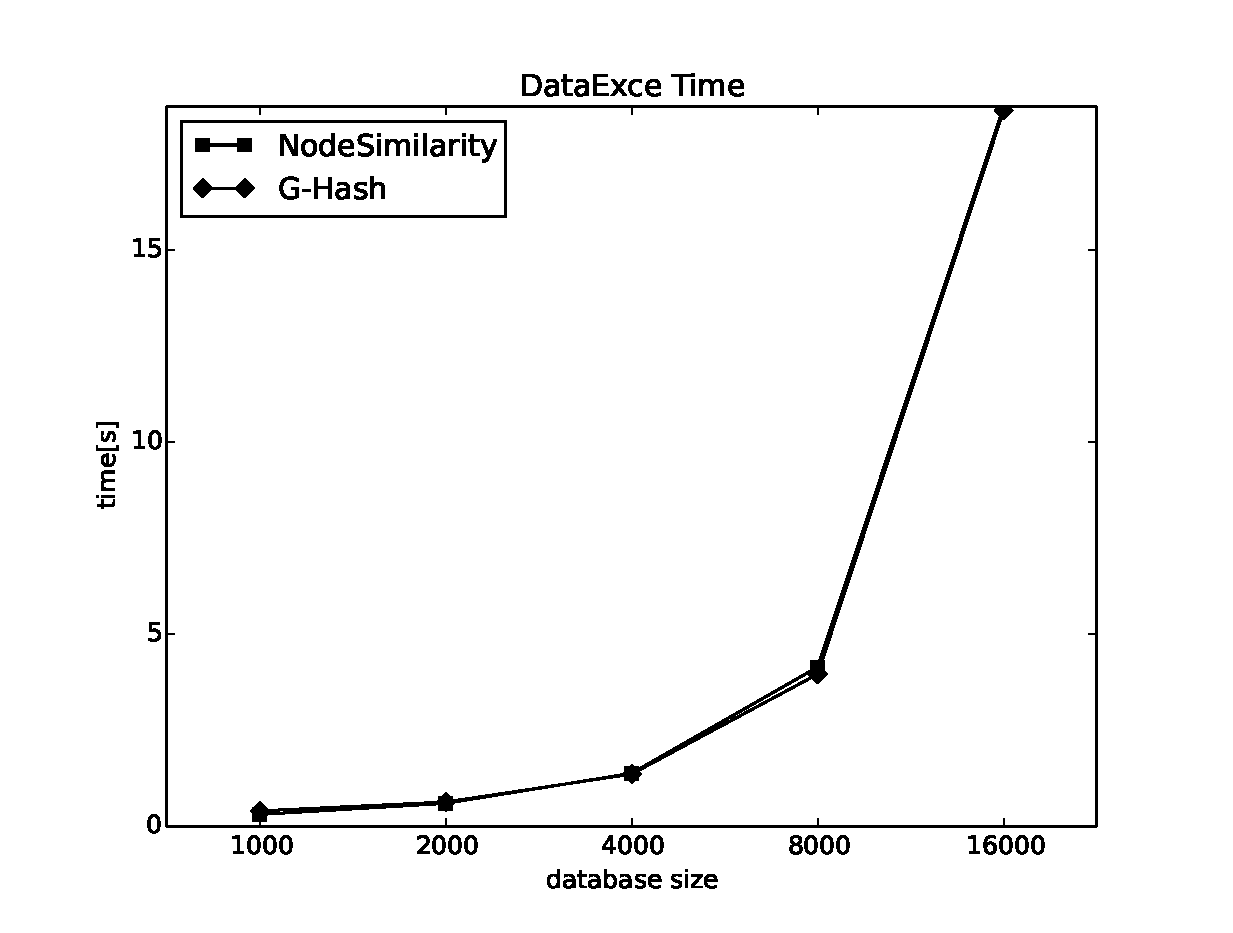
\includegraphics[width=\textwidth]{../figures/THC/G-Hashcomapre}
    \caption{查询时间对比图}
    \label{fg:ghashtime}
\end{figure}

实验结果如图\ref{fg:ghashtime}所示,可以看出节点相似度算法与G-Hash算法在线查询时间基本一致,说明其性能不输于G-Hash算法,但是编码难度大大降低。由于近似搜索的精度并不好定义,因此我们没有给出精度的对比图。不过由于G-Hash靠哈希函数获得相似节点,具有局限性。而本算法则是完全计算所有节点相似度,显然更加可靠。

\ifx\allfiles\undefined
%\bibliographystyle{unsrt}
\bibliography{main}
\end{document}
\fi
    \ifx\allfiles\undefined
\documentclass{XDBAthesis}
\def\pictures{}
\begin{document}
\else
\fi
\chapter{总结与展望}
\label{chap:future}
本章作为全文的最后一章,将对本文的所述内容进行总结,并对下一步的研究工作给出一些意见。
\section{本文总结}
\todo{根据绪论补充}
主要工作如下:
\begin{enumerate}
    \item 本文首先介绍了下图的基本定义,存储方法,图查询类型和一些经典的查询算法。
    \item 随后,我们对于图精确搜索提出了一种基于二次哈希开链法的搜索算法,有效避免了传统哈希方法冲突频发的问题,加速了整个查询过程。本文中,我们完整得介绍了这种算法,从数据库建库,到查询剪枝,直最后的子图同构检测,并通过实验证明了此算法确实可以加快整个查询过程。
    \item 然后,对于图相似性搜索我们提出了一种基于节点相似度的搜索算法。本算法与G-Hash算法大致相同,但重新定义了其核心部分——图相似度度量方法,使得编码复杂度大大降低,但同时效率又不低于G-Hash算法。本文中我们除了详细介绍了此算法原理,还给出了算法设计类图,并通过实验证明了此算法完全符合我们预期的目标——运行效率不低于G-Hash,甚至在某些情况下略好于G-Hash,但是编码难度大大下降。
\end{enumerate}

综上所述,本文对子图搜索方面做了一定基础性的研究,在认真研究了前人的经典算法基础上,进行了一些新的探索。
\section{进一步的工作}
但是,图数据查询仍是图数据管理中的一个重要领域,其中仍有一些问题需要继续去研究与改进。在未来的研究过程中,可以从以下几个方面入手:
\begin{enumerate}
    \item 目前,时时刻刻产生着大量的图数据信息,如何在图数据库中有效存储,在内存中以何种结构存储图数据,如何用固定的磁盘页面存储不同规模尺寸的图数据,又如何对图数据进行压缩表示,这些基本的物理存储问题将直接决定I/O操作的用时。而在实际中对图的存取又是非常频繁的,所以如果能解决存储问题,那么必然能提高整体查询效率。
    \item 除了物理存储,逻辑索引显得更为重要,如何高效索引,如何进行维护和更新,这些都是亟待解决的问题。特别是图索引的维护与更新,由于目前大量算法都处于理论阶段而并非实际运用,所以都没有涉及动态维护与更新。但是随着图数据越来越为重要,实际中对图的应用也日益增多。如果能解决这个问题,那么对图从实验室走到实际运用中将会是个强助力。
    \item 图查询的计算复杂度通常能达到指数级及以上,单线程的运算速度就成了图查询速度的瓶颈。因此考虑利用CPU/GPU异构并行或者多处理器并行,多机并行等也是一个不错的研究课题。
\end{enumerate}
\ifx\allfiles\undefined
%\bibliographystyle{unsrt}
\bibliography{main}
\end{document}
\fi
%    \appendix
%    
\chapter[本科生毕业设计论文撰写规范]{西安电子科技大学本科生毕业设计论文撰写规范}
\label{chap:requires}
\section{毕业设计(论文)的总体要求}
撰写论文应简明扼要,一般不少于15000字(外语专业可适当减少,但不得少于10000单词,且须全部用外语书写)。

\section{毕业设计(论文)的编写格式}
每一章、节的格式和版面要求整齐划一、层次清楚。其中:
\begin{itemize}
  \item 论文用纸:统一用A4纸,与论文封皮,任务书,工作计划,成绩考核表一致。
  \item 章的标题:如:``摘要''、``目录''、``第一章''、``附录''等,黑体,三号,居中排列。
  \item 节的标题:如:``2.1  认证方案''、``9.5  小结''等,宋体,四号,居中排列。
  \item 正文:中文为宋体,英文为``Times News Roman'',小四号。正文中的图名和表名,宋体,五号。
  \item 页眉:宋体五号,居中排列。左面页眉为论文题目,右面页眉为章次和章标题。页眉底划线的宽度为0.75磅。
  \item 页码:宋体小五号,排在页眉行的最外侧,不加任何修饰。
\end{itemize}

\section{毕业设计(论文)的前置部分}
毕业设计(论文)的前置部分包括封面、中英文摘要、目录等。
\subsection{封面及打印格式}
\begin{itemize}
  \item 学号:按照学校的统一编号,在右上角正确打印自己的学号,宋体,小四号,加粗。
  \item 题目:题目应和任务书的题目一致,黑体,三号。
  \item 学院、专业、班级、学生姓名和导师姓名职称等内容,宋体,小三号,居中排列。
\end{itemize}

\subsection{中英文摘要及关键词}
摘要是关于论文的内容不加注释和评论的简短陈述,具有独立性和自含性。它主要是
简要说明研究工作的目的、方法、结果和结论,重点说明本论文的成果和新见解。关键词
是为了文献标引工作从论文中选取出来用以表示全文主题内容信息的术语。
\begin{enumerate}
  \item 中文摘要,宋体小四号,一般为300字;英文摘要,``Times News Roman''字
体,小四号,一般为300个实词。摘要中不宜出现公式、非公用的符号、术语等。
  \item 每篇论文选取3 \~{} 5个关键词,中文为黑体小四号,英文为``Times News Roman''字体加粗,小四号。关键词排列在摘要的左下方一行,起始格式为:``\textbf{关键词}:
      ''和``\textbf{Keyword:}''。具体的各个关键词以均匀间隔排列,之间不加任何分隔符号。
\end{enumerate}

\section{目录}
按照论文的章、节、附录等前后顺序,编写序号、名称和页码。目录页排在中英文摘要之后,主体部分必
须另页右面开始,全文以右页为单页页码。

\section{毕业设计(论文)的主体部分}
毕业设计(论文)的主体部分包括引言(绪论)、正文、结论、结束语、致谢、参考文献。
\subsection{绪论}
作为论文的开端,简要说明作者所做工作的目的、范围、国内外进展情况、前人研究成果、
本人的设想、研究方法等。
\subsection{正文} 为毕业设计(论文)的核心部分,包括理论分析、数据资料、实验方法、结果、本人的论点和结
论等内容,还要附有各种有关的图表、照片、公式等。要求理论正确、逻辑清楚、层次分明、文字流畅、数据真实可
靠,公式推导和计算结果无误,图表绘制要少而精。
\begin{description}
  \item[图] 包括曲线图、示意图、流程图、框图等。图序号一律用阿拉伯数字分章依序编码,如:图1.3、图2.11。每一图应有简短确切的
      图名,连同图序号置于图的正下方。图中坐标上标注的符号和缩略词必须与正文中一致。
  \item[表] 包括分类项目和数据,一般要求分类项目由左至右横排,数据从上到下竖列。分类项目横排中必须标明符号或单位,竖列的数据栏中不宜出现``同上'' 、``同左''等类似词语,一律填写具体的数字或文字。表序号一律用阿拉伯数字分章依序编码,如:表2.5、表10.3。每一表应有简短确切的题名,
      连同表序号置于表的正上方。
  \item[公式] 正文中的公式、算式、方程式等必须编排序号,序号一律用阿拉伯数字分章依序编码,如:式(3-32)、式(6-21)。对于较长的公式,另行居中横排,只可在符号处(如:+、-、*、/、$<$、 $>$等)转行。公式序号标注于该式所在行(当有续行时,应标注于最后 一行)的最右边。连续性的公式在``=''处排列整齐。大于999的整数或多于三位的小数,一律用半个阿拉伯数字符的小间隔分开;小于1的数应将0置于小数点之前。
  \item[计量单位] 单位名称和符号的书写方式一律采用国际通用符号。
\end{description}

\subsection{结论}
是对主体的最终结论,应准确、完整、精炼。阐述作者创造性工作在本研究领域的地位和作用,对存在的问题和不足应给予客观的说明,也可提出进一步的设想。

\subsection{致谢}
对协助完成论文研究工作的单位和个人表示感谢。

\subsection{参考文献}
在学位论文中引用参考文献时,引出处右上角用方括号标注阿拉伯数字编排的序号(必须与参考文献一致)。参考文献的排列格
式分为:
\begin{description}
  \item[专著类的文献] [序号]  作者 . 专著名称.  版本. 出版地:出版者,出版年. 参考的页码。
  \item[期刊类的文献] 作者 . 文献名. 期刊名称.  年 , 月,  卷(期). 页码。
\end{description}
其中作者采用姓在前、名在后的形式。当作者超过三个时,只著录前三个人,其后
加``等''字即可。

\section{毕业设计(论文)的附录部分}
附录是作为学位论文主体的补充,包括下列内容:
\begin{enumerate}
  \item 正文中过于冗长的公式推导;
  \item 为读者阅读方便所需要的辅助性的数学工作或带有重复性的图表;
  \item 由于过分冗长而不宜在正文中出现的计算机程序清单;
  \item 对于一般读者并非必要阅读,但对本专业同行有参考价值的资料。
  \item 附录编于正文后,与正文连续编页码,每一附录均另页起。
  \item 附录依次用大写正体A,B,C……编序号,黑体,三号。如:附录A。
  \item 附录中的图、表、式、参考文献等与正文分开,用阿拉伯数字另行编序号,注意在数码前冠以附录的
      序码。如:图A1;表B2;式(C-3);文献[D5]。
\end{enumerate}
\section{毕业设计(论文)的打印规格}
论文正文页面和版面的设置规格:论文正文双面打印,为了便于装订、复制,要求每页纸的四周留有足够的空白边缘。以WORD97为例:

页面设置数据为:上3厘米、下2厘米、内侧3厘米、外侧2厘米;装订线 -- 1厘米;页眉  - 2厘米;  页脚 - 1厘米。

版面设置数据为:文字的行间距 - 1. 5倍 ;  公式的行间距 - 1. 5倍字符间距 - 标准;页码数据-对称页边距。

\section{毕业设计(论文)的装订说明}
毕业设计(论文)要求以A4纸的标准,按照下列顺序装订。外文资料翻译原文及译文另册装订,格式参照论文对应内容格式要求。

\begin{enumerate}
  \item 封面
  \item 任务书
  \item 工作计划
  \item 中期检查表
  \item 成绩考核登记表
  \item 中、外论文摘要
  \item 目录
  \item 引言
  \item 论文
  \item 结论
  \item 结束语
  \item 参考文献
  \item 附录
\end{enumerate}












%%----------------- 附件部分 ----------------- %%
    \backmatter
    \ifx\allfiles\undefined
\documentclass{XDBAthesis}
\def\pictures{}
\begin{document}
\else
\fi

\begin{thanks}

毕业论文暂告收尾,这也意味着我在西安电子科技大学的四年的学习生活既将结束。回首既往,自己一生最宝贵的时光能于这样的校园之中,能在众多学富五车、才华横溢的老师们的熏陶下度过,实是荣幸之极。在这四年的时间里,我在学习上和思想上都受益非浅。这除了自身努力外,与各位老师、同学和朋友的关心、支持和鼓励是分不开的。

首先感谢霍红卫教授的指导,霍老师在我论文写作期间给了我莫大的帮助。从选题到构思,研究,撰写,每一步都倾注了霍老师大量的心血。

其次感谢陈晓阳学长,每次在我迷茫时都给我指明了方向。特别是研究遇到一些瓶颈时,陈学长都会用其丰富的经验帮我度过。

感谢ShaSha教授,提供了GraphGrep源代码。

时间的仓促及自身专业水平的不足,整篇论文肯定存在尚未发现的缺点和错误。
恳请阅读此篇论文的老师、同学,多予指正,不胜感激!


\end{thanks}

\ifx\allfiles\undefined
%\bibliographystyle{unsrt}
\bibliography{main}
\end{document}
\fi
%    
\fontsize{10.5pt}{10.5pt}\selectfont
\begin{thebibliography}{10}

\bibitem{site:ctex}
 http://www.ctex.org


\bibitem{lshort-cn}
\CTeX{}~翻译小组.
\newblock {lshort~中文版~}.
\newblock (2003)


\bibitem{deng:01a}
{邓建松,~彭冉冉,~陈长松}.
\newblock {\LaTeXe{}~科技排版指南}.
\newblock 科学出版社,~书号:~7-03-009239-2/TP.1516, 北京, (2001).

\bibitem{wang:00a}
王磊.
\newblock {\LaTeXe{}~插图指南}.
\newblock (2000).

\bibitem{zhang:03a}
张林波.
\newblock {于新版~CCT~的说明}.
\newblock (2003).

\bibitem{knuth86e}
Donald~E, Knuth.
\newblock {Computer Modern Typefaces}, volume~E of {Computers and
  Typesetting}.
\newblock Addison-Wesley, Reading, Massachusetts, (1986).

\bibitem{knuth86d}
Donald~E. Knuth.
\newblock {{METAFONT}: The Program}, volume~D of {Computers and
  Typesetting}.
\newblock Addison-Wesley, Reading, Massachusetts, (1986).

\bibitem{knuth86c}
Donald~E. Knuth.
\newblock {The {METAFONT}book}, volume~C of {Computers and
  Typesetting}.
\newblock Addison-Wesley, Reading, Massachusetts, (1986).

\bibitem{knuth86b}
Donald~E. Knuth.
\newblock {{\TeX}: The Program}, volume~B of { Computers and
  Typesetting}.
\newblock Addison-Wesley, Reading, Massachusetts, (1986).

\bibitem{knuth86a}
Donald~E. Knuth.
\newblock {The {TeX}book}, volume~A of {Computers and Typesetting}.
\newblock Addison-Wesley, Reading, Massachusetts, (1986).

\bibitem{lamport85a}
Leslie Lamport.
\newblock {{\LaTeX} --- A Document Preparation System: User's Guide and
  Reference Manual}.
\newblock Addison-Wesley, Reading, Massachusetts, 2nd edition, (1985).

\end{thebibliography}

    
\bibliographystyle{unsrt}
\bibliography{main}
\end{document}
